\clearpage
\cleardoublepage

\chapter{数学基础}

\section{引言}

神经网络建立在坚实的数学基础之上，结合了线性代数、微积分、概率论和优化理论。本章提供了理解神经网络如何学习和预测的基本数学先验知识。我们将在深度学习应用的背景下介绍这些主题，提供理论洞察和实践直觉。

神经网络的数学可以看作是非线性激活函数的线性变换组合，通过基于梯度的方法进行优化。理解这个框架需要熟练掌握向量和矩阵运算、多元函数微分以及随机优化。

\section{线性代数}

线性代数提供了在神经网络中表示和操作数据的语言。神经网络基本上通过线性变换（矩阵乘法）与非线性激活函数结合来运作。

\subsection{向量与矩阵}

向量是有序的数字集合，可以表示 $n$ 维空间中的一个点。在神经网络中，输入数据、隐藏表示和参数都表示为向量或更高维的张量。

\begin{定义}[向量]
向量 $\mathbf{x} \in \mathbb{R}^n$ 是 $n$ 个实数的有序元组：
\begin{equation}
\mathbf{x} = \begin{bmatrix} x_1 \\ x_2 \\ \vdots \\ x_n \end{bmatrix} = (x_1, x_2, \ldots, x_n)^\top
\end{equation}
其中 $x_i$ 表示向量的第 $i$ 个分量。
\end{定义}

\begin{定义}[矩阵]
矩阵 $\mathbf{A} \in \mathbb{R}^{m \times n}$ 是 $m$ 行 $n$ 列的二维数组：
\begin{equation}
\mathbf{A} = \begin{bmatrix}
a_{11} & a_{12} & \cdots & a_{1n} \\
a_{21} & a_{22} & \cdots & a_{2n} \\
\vdots & \vdots & \ddots & \vdots \\
a_{m1} & a_{m2} & \cdots & a_{mn}
\end{bmatrix}
\end{equation}
其中 $a_{ij}$ 表示第 $i$ 行第 $j$ 列的元素。
\end{定义}

\begin{示例}[神经网络层作为矩阵运算]
单层全连接神经网络执行以下运算：
\begin{equation}
\mathbf{y} = \mathbf{W}\mathbf{x} + \mathbf{b}
\end{equation}
其中：
\begin{itemize}
    \item $\mathbf{x} \in \mathbb{R}^{d_{in}}$ 是输入向量
    \item $\mathbf{W} \in \mathbb{R}^{d_{out} \times d_{in}}$ 是权重矩阵
    \item $\mathbf{b} \in \mathbb{R}^{d_{out}}$ 是偏置向量
    \item $\mathbf{y} \in \mathbb{R}^{d_{out}}$ 是输出向量
\end{itemize}
如果 $d_{in} = 784$（MNIST 图像）且 $d_{out} = 128$，则 $\mathbf{W}$ 包含 $784 \times 128 = 100,352$ 个参数。
\end{示例}

\subsection{矩阵运算}

\begin{itemize}
    \item \textbf{矩阵加法：} $\mathbf{C} = \mathbf{A} + \mathbf{B}$，其中 $c_{ij} = a_{ij} + b_{ij}$
    \item \textbf{标量乘法：} $c\mathbf{A}$，其中每个元素都乘以 $c$
    \item \textbf{矩阵乘法：} $\mathbf{C} = \mathbf{AB}$，其中 $c_{ij} = \sum_{k} a_{ik}b_{kj}$
    \item \textbf{转置：} $(\mathbf{A}^\top)_{ij} = a_{ji}$
    \item \textbf{逐元素（哈达玛）乘积：} $(\mathbf{A} \odot \mathbf{B})_{ij} = a_{ij} \cdot b_{ij}$
\end{itemize}

\begin{性质}[矩阵乘法性质]
对于适当维度的矩阵 $\mathbf{A}$、$\mathbf{B}$ 和 $\mathbf{C}$：
\begin{align}
\mathbf{A}(\mathbf{BC}) &= (\mathbf{AB})\mathbf{C} \quad \text{（结合律）} \\
\mathbf{A}(\mathbf{B} + \mathbf{C}) &= \mathbf{AB} + \mathbf{AC} \quad \text{（分配律）} \\
(\mathbf{AB})^\top &= \mathbf{B}^\top \mathbf{A}^\top \quad \text{（乘积的转置）}
\end{align}
注意：一般情况下 $\mathbf{AB} \neq \mathbf{BA}$（不可交换）。
\end{性质}

\subsection{范数}

范数衡量向量和矩阵的``大小''或``长度''。

\begin{定义}[向量范数]
对于向量 $\mathbf{x} \in \mathbb{R}^n$：
\begin{itemize}
    \item $L_1$ 范数（曼哈顿范数）：$\|\mathbf{x}\|_1 = \sum_{i=1}^{n} |x_i|$
    \item $L_2$ 范数（欧几里得范数）：$\|\mathbf{x}\|_2 = \sqrt{\sum_{i=1}^{n} x_i^2}$
    \item $L_p$ 范数：$\|\mathbf{x}\|_p = \left(\sum_{i=1}^{n} |x_i|^p\right)^{1/p}$
    \item $L_\infty$ 范数（最大范数）：$\|\mathbf{x}\|_\infty = \max_i |x_i|$
\end{itemize}
\end{定义}

在神经网络中，$L_2$ 范数常用于正则化（权重衰减），而 $L_1$ 范数促进稀疏性。

\begin{示例}[权重衰减正则化]
权重衰减向损失函数添加惩罚项：
\begin{equation}
\mathcal{L}_{reg}(\mathbf{W}) = \mathcal{L}(\mathbf{W}) + \lambda \|\mathbf{W}\|_F^2
\end{equation}
其中 $\|\mathbf{W}\|_F = \sqrt{\sum_{i,j} w_{ij}^2}$ 是 Frobenius 范数（展平矩阵的 $L_2$ 范数）。
\end{示例}

\subsection{特征值与奇异值}

特征值和奇异值对于理解线性变换、维度约简和网络分析至关重要。

\begin{定义}[特征值与特征向量]
对于方阵 $\mathbf{A} \in \mathbb{R}^{n \times n}$，如果存在标量 $\lambda$ 和非零向量 $\mathbf{v}$ 使得：
\begin{equation}
\mathbf{A}\mathbf{v} = \lambda \mathbf{v}
\end{equation}
则称 $\lambda$ 为特征值，$\mathbf{v}$ 为对应的特征向量。
\end{定义}

\begin{定义}[奇异值分解]
对于任意矩阵 $\mathbf{A} \in \mathbb{R}^{m \times n}$，奇异值分解（SVD）为：
\begin{equation}
\mathbf{A} = \mathbf{U}\Sigma\mathbf{V}^\top
\end{equation}
其中：
\begin{itemize}
    \item $\mathbf{U} \in \mathbb{R}^{m \times m}$ 和 $\mathbf{V} \in \mathbb{R}^{n \times n}$ 是正交矩阵
    \item $\Sigma \in \mathbb{R}^{m \times n}$ 是包含奇异值 $\sigma_1 \geq \sigma_2 \geq \cdots \geq 0$ 的对角矩阵
\end{itemize}
奇异值与特征值的关系为 $\sigma_i = \sqrt{\lambda_i(\mathbf{A}^\top\mathbf{A})}$。
\end{定义}

SVD 对主成分分析（PCA）至关重要，PCA 用于理解神经网络表示的维度。

\subsubsection{为什么 SVD 很重要：几何解释}

为了理解 SVD 的基础性，考虑矩阵 $\mathbf{A}$ 的几何作用。方程 $\mathbf{y} = \mathbf{A}\mathbf{x}$ 可以通过 SVD 分解为三个顺序变换：
\begin{enumerate}
    \item $\mathbf{V}^\top$：将输入向量旋转（或反射）到``右奇异基''。
    \item $\Sigma$：沿每个轴按相应奇异值 $\sigma_i$ 缩放。
    \item $\mathbf{U}$：旋转到输出空间的``左奇异基''。
\end{enumerate}
这个几何视图揭示了奇异值 $\sigma_1 \geq \sigma_2 \geq \cdots \geq 0$ 精确描述了 $\mathbf{A}$ 沿每个主方向拉伸空间的程度。在神经网络中，一层的权重矩阵 $\mathbf{W}$ 正好对输入激活执行这种变换。

\begin{figure}[htbp]
    \centering
    \begin{tikzpicture}[scale=0.9]
        \begin{axis}[
            xlabel={$\sigma_1$（奇异值）},
            ylabel={累积方差解释率},
            xmin=0, xmax=10,
            ymin=0, ymax=1.05,
            width=10cm,
            height=6cm,
            legend pos=south east,
            grid=major
        ]
            \addplot[thick, blue, mark=*, mark size=1.5pt] coordinates {
                (9.5, 0.35) (7.2, 0.58) (4.1, 0.72) (2.8, 0.82)
                (1.9, 0.89) (1.2, 0.93) (0.7, 0.96) (0.4, 0.98)
                (0.2, 0.99) (0.1, 1.0)
            };
            \addlegendentry{累积方差}
            \addplot[dashed, red, thick] coordinates {(0, 0.9) (10, 0.9)};
            \addlegendentry{90\% 阈值}
        \end{axis}
    \end{tikzpicture}
    \caption[奇异值谱]{神经网络权重矩阵的典型奇异值谱。大多数方差由前几个奇异值捕获，这促使人们使用低秩近似。}
    \label{fig:svd_spectrum}
\end{figure}

\subsubsection{低秩近似：Eckart--Young 定理}

SVD 在深度学习中最强大的应用之一是低秩近似。给定秩-$r$ 近似 $\hat{\mathbf{A}}_r = \sum_{i=1}^{r} \sigma_i \mathbf{u}_i \mathbf{v}_i^\top$，Eckart--Young 定理保证：

\begin{定理}[Eckart--Young--Mirsky，1936/1949]
对于任意矩阵 $\mathbf{A} \in \mathbb{R}^{m \times n}$，其 SVD 为 $\mathbf{A} = \mathbf{U}\Sigma\mathbf{V}^\top$，在谱范数和 Frobenius 范数意义下的最佳秩-$r$ 近似由保留前 $r$ 个奇异值给出：
\begin{equation}
\hat{\mathbf{A}}_r = \arg\min_{\text{rank}(\mathbf{B}) \leq r} \|\mathbf{A} - \mathbf{B}\|_F = \sum_{i=1}^{r} \sigma_i \mathbf{u}_i \mathbf{v}_i^\top
\end{equation}
近似误差为 $\|\mathbf{A} - \hat{\mathbf{A}}_r\|_F = \sqrt{\sum_{i=r+1}^{\min(m,n)} \sigma_i^2}$。
\end{定理}

这个定理支撑了诸如 \textbf{LoRA}（低秩适应）等现代技术 \cite{hu2021lora}，用于高效微调大语言模型，其中权重更新 $\Delta\mathbf{W}$ 被参数化为 $\mathbf{B}\mathbf{A}$ 的乘积，秩 $r \ll \min(m, n)$，将可训练参数从 $mn$ 减少到 $(m + n)r$。

\subsubsection{特征分解与谱定理}

对于对称矩阵（作为优化中的 Hessian 矩阵 $\mathbf{H}$ 经常出现），特征分解采用一种特殊且简化的形式：

\begin{定理}[谱定理]
对于任意实对称矩阵 $\mathbf{A} \in \mathbb{R}^{n \times n}$（$\mathbf{A} = \mathbf{A}^\top$），存在正交矩阵 $\mathbf{Q}$ 和对角矩阵 $\Lambda$ 使得：
\begin{equation}
\mathbf{A} = \mathbf{Q}\Lambda\mathbf{Q}^\top = \sum_{i=1}^{n} \lambda_i \mathbf{q}_i \mathbf{q}_i^\top
\end{equation}
其中 $\lambda_1 \geq \lambda_2 \geq \cdots \geq \lambda_n$ 是实特征值，$\mathbf{q}_i$ 是正交特征向量。
\end{定理}

损失函数的 Hessian $\mathbf{H} = \nabla^2 \mathcal{L}(\boldsymbol{\theta})$ 始终是对称的（根据混合偏导数相等的 Clairaut 定理）。其特征值决定了损失表面的局部几何：
\begin{itemize}
    \item 所有 $\lambda_i > 0$：局部最小值（正定）
    \item 所有 $\lambda_i < 0$：局部最大值（负定）
    \item 混合符号：鞍点（不定）
\end{itemize}

\subsubsection{条件数与数值稳定性}

矩阵的条件数衡量 $\mathbf{A}\mathbf{x} = \mathbf{b}$ 的解对 $\mathbf{b}$ 中扰动的敏感程度：

\begin{定义}[条件数]
矩阵 $\mathbf{A}$（相对于 $L_2$ 范数）的条件数为：
\begin{equation}
\kappa(\mathbf{A}) = \|\mathbf{A}\|_2 \cdot \|\mathbf{A}^{-1}\|_2 = \frac{\sigma_{\max}(\mathbf{A})}{\sigma_{\min}(\mathbf{A})}
\end{equation}
对于对称正定矩阵，$\kappa(\mathbf{A}) = \lambda_{\max} / \lambda_{\min}$。
\end{定义}

在梯度下降中，Hessian $\kappa(\mathbf{H})$ 的条件数直接限制收敛速度。对于二次目标 $\mathcal{L}(\boldsymbol{\theta}) = \frac{1}{2}\boldsymbol{\theta}^\top \mathbf{H}\boldsymbol{\theta} - \mathbf{b}^\top\boldsymbol{\theta}$，学习率为 $\alpha$ 的梯度下降当且仅当以下条件成立时收敛：
\begin{equation}
0 < \alpha < \frac{2}{\lambda_{\max}}
\end{equation}
最优学习率为 $\alpha^* = \frac{2}{\lambda_{\max} + \lambda_{\min}}$，给出每轮收敛速度：
\begin{equation}
\left(\frac{\kappa(\mathbf{H}) - 1}{\kappa(\mathbf{H}) + 1}\right)^2
\end{equation}
当 $\kappa(\mathbf{H}) \gg 1$（病态）时，收敛变得极慢——这是像 Adam（第 7 章）这样的自适应优化器的根本动机，它有效地沿每个维度重新缩放梯度。

\begin{figure}[htbp]
    \centering
    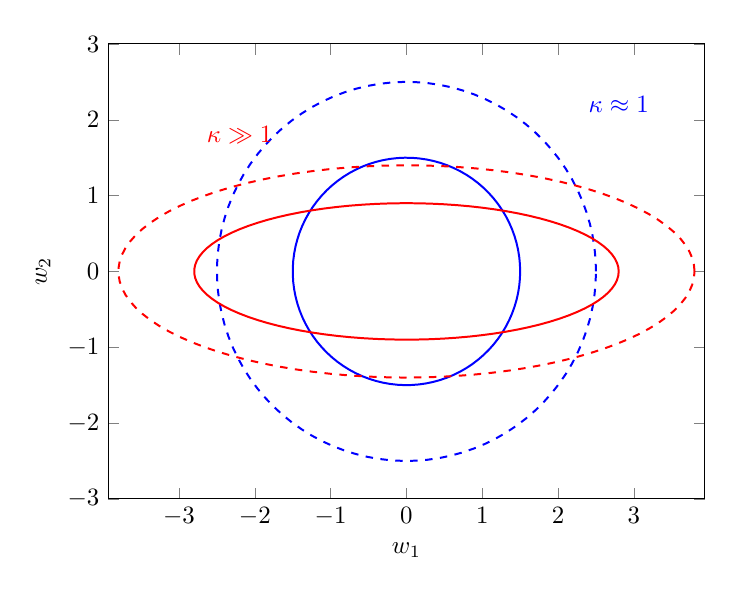
\begin{tikzpicture}[scale=0.9]
        \begin{axis}[
            xlabel={$w_1$},
            ylabel={$w_2$},
            width=10cm,
            height=8cm,
            axis equal,
            xmin=-3, xmax=3,
            ymin=-3, ymax=3,
        ]
            % 良态（kappa ~ 1）
            \addplot[blue, thick, domain=0:360, samples=100]
                ({1.5*cos(x)}, {1.5*sin(x)});
            \addplot[blue, thick, dashed, domain=0:360, samples=100]
                ({2.5*cos(x)}, {2.5*sin(x)});
            \node[blue] at (axis cs:2.8, 2.2) {$\kappa \approx 1$};
            
            % 病态（kappa ~ 10）
            \addplot[red, thick, domain=0:360, samples=100]
                ({2.8*cos(x)}, {0.9*sin(x)});
            \addplot[red, thick, dashed, domain=0:360, samples=100]
                ({3.8*cos(x)}, {1.4*sin(x)});
            \node[red] at (axis cs:-2.2, 1.8) {$\kappa \gg 1$};
        \end{axis}
    \end{tikzpicture}
    \caption[条件数与损失等高线]{良态（圆形，$\kappa \approx 1$）和病态（椭圆形，$\kappa \gg 1$）问题的损失等高线。梯度下降在病态地形上呈锯齿状。}
    \label{fig:condition_number}
\end{figure}

\subsubsection{正定矩阵与 Cholesky 分解}

\begin{定义}[正定]
如果对称矩阵 $\mathbf{A}$ 对所有非零 $\mathbf{x}$ 满足 $\mathbf{x}^\top \mathbf{A}\mathbf{x} > 0$，则它是正定的。
\end{定义}

对于协方差矩阵（始终是半正定的），Cholesky 分解提供了高效的因式分解：

\begin{定理}[Cholesky 分解]
对于任意对称正定 $\mathbf{A} \in \mathbb{R}^{n \times n}$：
\begin{equation}
\mathbf{A} = \mathbf{L}\mathbf{L}^\top
\end{equation}
其中 $\mathbf{L}$ 是对角元素为正的下三角矩阵。计算需要 $\frac{n^3}{6}$ FLOPs，是 LU 分解的一半。
\end{定理}

Cholesky 分解对于以下方面至关重要：
\begin{itemize}
    \item \textbf{从多元高斯分布采样：} 如果 $\mathbf{x} \sim \mathcal{N}(\boldsymbol{\mu}, \boldsymbol{\Sigma})$，则 $\mathbf{x} = \boldsymbol{\mu} + \mathbf{L}\mathbf{z}$，其中 $\mathbf{z} \sim \mathcal{N}(\mathbf{0}, \mathbf{I})$ 且 $\boldsymbol{\Sigma} = \mathbf{L}\mathbf{L}^\top$。
    \item \textbf{卡尔曼滤波器}和概率深度学习中的\textbf{变分推断}。
    \item 优化子程序中\textbf{求解线性系统} $\mathbf{A}\mathbf{x} = \mathbf{b}$。
\end{itemize}

\subsubsection{行列式、迹与 Jacobian 行列式}

两个在深度学习中经常出现的矩阵标量总结：

\begin{性质}[关键矩阵性质]
对于具有特征值 $\lambda_1, \ldots, \lambda_n$ 的 $n \times n$ 矩阵 $\mathbf{A}$：
\begin{align}
\det(\mathbf{A}) &= \prod_{i=1}^{n} \lambda_i = \text{符号体积缩放因子} \\
\text{tr}(\mathbf{A}) &= \sum_{i=1}^{n} \lambda_i = \sum_{i=1}^{n} a_{ii} \\
\det(\mathbf{A}) &= \exp(\text{tr}(\log \mathbf{A})) \quad \text{（矩阵对数恒等式）}
\end{align}
\end{性质}

\textbf{Jacobian 行列式}在归一化流和变分自编码器（VAE）中至关重要。如果 $\mathbf{y} = g(\mathbf{x})$ 是可逆变换，则根据变量变换公式：
\begin{equation}
p_{\mathbf{Y}}(\mathbf{y}) = p_{\mathbf{X}}(g^{-1}(\mathbf{y})) \cdot \left|\det \frac{\partial g^{-1}(\mathbf{y})}{\partial \mathbf{y}}\right| = p_{\mathbf{X}}(\mathbf{x}) \cdot \left|\det \frac{\partial g(\mathbf{x})}{\partial \mathbf{x}}\right|^{-1}
\end{equation}
归一化流设计 $g$ 使得行列式计算成本低廉，从而实现精确的似然评估。本书后面将讨论用于生成建模的变分自编码器和归一化流。

\subsection{张量}

神经网络，特别是卷积神经网络，在称为张量的高维数组上运作。

\begin{定义}[张量]
张量是向量和矩阵到更高维度的推广：
\begin{itemize}
    \item 0D 张量：标量
    \item 1D 张量：向量
    \item 2D 张量：矩阵
    \item 3D 张量：例如形状为 $(H, W, C)$ 的 RGB 图像
    \item 4D 张量：形状为 $(N, H, W, C)$ 的图像批次
    \item 5D 张量：形状为 $(D, H, W, C)$ 的体积
\end{itemize}
\end{定义}

\begin{示例}[CNN 中的张量形状]
对于 $N$ 张大小为 $H \times W$、3 通道（RGB）的彩色图像批次：
\begin{itemize}
    \item 输入张量：$\mathbf{X} \in \mathbb{R}^{N \times H \times W \times 3}$
    \item 与 $C$ 个滤波器卷积后：$\mathbf{Y} \in \mathbb{R}^{N \times H' \times W' \times C}$
\end{itemize}
PyTorch 约定：$(N, C, H, W)$
TensorFlow 约定：$(N, H, W, C)$
\end{示例}

\section{微积分}

微积分，特别是微分，对于理解神经网络通过基于梯度的优化进行学习至关重要。

\subsection{导数与梯度}

\begin{定义}[导数]
函数 $f: \mathbb{R} \to \mathbb{R}$ 在点 $x$ 处的导数定义为：
\begin{equation}
f'(x) = \frac{df}{dx} = \lim_{h \to 0} \frac{f(x + h) - f(x)}{h}
\end{equation}
\end{定义}

\begin{定义}[梯度]
对于标量函数 $f: \mathbb{R}^n \to \mathbb{R}$，梯度是偏导数的向量：
\begin{equation}
\nabla f(\mathbf{x}) = \begin{bmatrix}
\frac{\partial f}{\partial x_1} \\
\frac{\partial f}{\partial x_2} \\
\vdots \\
\frac{\partial f}{\partial x_n}
\end{bmatrix}
\end{equation}
梯度指向最陡上升方向。
\end{定义}

\begin{性质}[微分规则]
\begin{itemize}
    \item 和规则：$\frac{d}{dx}(f + g) = f' + g'$
    \item 乘积规则：$\frac{d}{dx}(fg) = f'g + fg'$
    \item 链式规则：$\frac{d}{dx}f(g(x)) = f'(g(x)) \cdot g'(x)$
    \item 商规则：$\frac{d}{dx}\left(\frac{f}{g}\right) = \frac{f'g - fg'}{g^2}$
\end{itemize}
\end{性质}

\begin{示例}[神经网络中的链式规则]
对于双层网络 $f(\mathbf{x}) = \mathbf{W}_2(\mathbf{W}_1\mathbf{x} + \mathbf{b}_1) + \mathbf{b}_2$，梯度计算广泛使用链式规则。如果我们想要损失 $\mathcal{L}$ 关于 $\mathbf{W}_1$ 的梯度 $\frac{\partial \mathcal{L}}{\partial \mathbf{W}_1}$，有：
\begin{equation}
\frac{\partial \mathcal{L}}{\partial \mathbf{W}_1} = \frac{\partial \mathcal{L}}{\partial \mathbf{z}_2} \cdot \frac{\partial \mathbf{z}_2}{\partial \mathbf{z}_1} \cdot \frac{\partial \mathbf{z}_1}{\partial \mathbf{W}_1}
\end{equation}
其中 $\mathbf{z}_1 = \mathbf{W}_1\mathbf{x} + \mathbf{b}_1$ 且 $\mathbf{z}_2 = \mathbf{W}_2\mathbf{z}_1 + \mathbf{b}_2$。
\end{示例}

\subsection{高阶导数}

\begin{定义}[Hessian 矩阵]
对于函数 $f: \mathbb{R}^n \to \mathbb{R}$，Hessian 矩阵包含所有二阶偏导数：
\begin{equation}
\mathbf{H} = \nabla^2 f(\mathbf{x}) = \begin{bmatrix}
\frac{\partial^2 f}{\partial x_1^2} & \frac{\partial^2 f}{\partial x_1 \partial x_2} & \cdots \\
\frac{\partial^2 f}{\partial x_2 \partial x_1} & \frac{\partial^2 f}{\partial x_2^2} & \cdots \\
\vdots & \vdots & \ddots
\end{bmatrix}
\end{equation}
如果所有二阶导数连续，则 Hessian 是对称的。
\end{定义}

Hessian 用于牛顿法和理解损失景观的曲率。

\subsubsection{泰勒展开：理论桥梁}

泰勒展开是连接一阶和二阶优化方法的单一最重要的数学工具。对于围绕点 $\mathbf{a}$ 的二次可微函数 $f: \mathbb{R}^n \to \mathbb{R}$：

\begin{定义}[多元泰勒展开]
\begin{align}
f(\mathbf{a} + \boldsymbol{\delta}) &= f(\mathbf{a}) + \nabla f(\mathbf{a})^\top \boldsymbol{\delta} + \frac{1}{2}\boldsymbol{\delta}^\top \mathbf{H}(\mathbf{a})\boldsymbol{\delta} + \mathcal{O}(\|\boldsymbol{\delta}\|^3)
\end{align}
其中 $\nabla f(\mathbf{a})$ 是梯度，$\mathbf{H}(\mathbf{a}) = \nabla^2 f(\mathbf{a})$ 是在 $\mathbf{a}$ 处求值的 Hessian。
\end{定义}

\textbf{这对神经网络的重要性：} 几乎所有优化理论都可以通过局部泰勒近似的视角来理解。

\begin{示例}[梯度下降作为一阶泰勒近似]
将 $\boldsymbol{\delta} = -\alpha \nabla f(\mathbf{a})$ 代入一阶展开：
\begin{equation}
f(\mathbf{a} - \alpha \nabla f(\mathbf{a})) \approx f(\mathbf{a}) - \alpha \|\nabla f(\mathbf{a})\|^2
\end{equation}
只要 $\alpha > 0$ 且线性近似有效——即 $\alpha$ 不是太大——这保证了下降。
\end{示例}

\begin{示例}[牛顿法作为二阶近似]
最小化二阶泰勒近似：
\begin{equation}
f(\mathbf{a} + \boldsymbol{\delta}) \approx f(\mathbf{a}) + \nabla f(\mathbf{a})^\top \boldsymbol{\delta} + \frac{1}{2}\boldsymbol{\delta}^\top \mathbf{H}\boldsymbol{\delta}
\end{equation}
令关于 $\boldsymbol{\delta}$ 的梯度为零：
\begin{equation}
\nabla f(\mathbf{a}) + \mathbf{H}\boldsymbol{\delta}^* = 0 \implies \boldsymbol{\delta}^* = -\mathbf{H}^{-1}\nabla f(\mathbf{a})
\end{equation}
这就是牛顿更新。它在最小值附近二次收敛，但每步需要 $\mathcal{O}(n^3)$ 进行矩阵求逆——对于具有数百万参数深度网络来说成本过高。现代拟牛顿法（L-BFGS）和近似二阶法（K-FAC、Shampoo）试图以可管理的成本捕获曲率信息。
\end{示例}

\subsubsection{凸性与损失景观}

凸性决定梯度下降是否能找到全局最小值：

\begin{定义}[凸函数]
如果函数 $f$ 对所有 $\mathbf{x}, \mathbf{y}$ 和 $\lambda \in [0,1]$ 满足：
\begin{equation}
f(\lambda \mathbf{x} + (1-\lambda)\mathbf{y}) \leq \lambda f(\mathbf{x}) + (1-\lambda)f(\mathbf{y})
\end{equation}
则 $f$ 是\textbf{凸函数}。
\end{定义}

\begin{定义}[强凸函数]
如果二次可微的 $f$ 是 $\mu$ 强凸的：
\begin{equation}
\nabla^2 f(\mathbf{x}) \succeq \mu \mathbf{I} \quad \text{（Hessian 的所有特征值 $\geq \mu > 0$）}
\end{equation}
\end{定义}

\textbf{坏消息：} 神经网络损失景观是\textbf{非凸的}——Hessian 到处都是既有正特征值又有负特征值。然而，一个引人注目的经验发现是\textbf{在过参数化网络中，大多数局部最小值具有相似的损失值} \cite{choriomanska2015loss}，主要挑战是鞍点而不是差的局部最小值。

\begin{table}[ht]
    \centering
    \caption{凸性性质及其对优化的影响}
    \begin{tabular}{L{3.5cm} L{4cm} L{5cm}}
        \toprule
        \textbf{性质} & \textbf{条件} & \textbf{含义} \\
        \midrule
        凸 & $\nabla^2 f \succeq 0$ & 所有局部最小值都是全局的 \\
        严格凸 & $\nabla^2 f \succ 0$ & 唯一全局最小值 \\
        $\mu$ 强凸 & $\nabla^2 f \succeq \mu\mathbf{I}$ & 线性收敛速度 \\
        $L$ 平滑 & $\|\nabla^2 f\| \leq L$ & $\alpha < 2/L$ 保证下降 \\
        PL 条件 & -- & 即使非凸也能线性收敛 \\
        \bottomrule
    \end{tabular}
\end{table}

Polyak--\L{}ojasiewicz（PL）条件是强凸性的放松，适用于一些非凸问题：
\begin{equation}
\frac{1}{2}\|\nabla f(\mathbf{x})\|^2 \geq \mu(f(\mathbf{x}) - f^*)
\end{equation}
其中 $f^*$ 是最优值。许多神经网络训练目标被推测近似满足此条件，这解释了尽管非凸性梯度下降为何经常找到好的解。

\subsubsection{Lipschitz 连续与梯度裁剪}

\begin{定义}[$L$-Lipschitz 连续]
如果函数 $f$ 是 $L$-Lipschitz 连续的：
\begin{equation}
|f(\mathbf{x}) - f(\mathbf{y})| \leq L\|\mathbf{x} - \mathbf{y}\| \quad \forall \mathbf{x}, \mathbf{y}
\end{equation}
对于可微 $f$，等价于 $\|\nabla f(\mathbf{x})\| \leq L$。
\end{定义}

在神经网络中，每层的 Lipschitz 常数限制输入的微小变化能多大程度上影响输出。对于线性层 $\mathbf{y} = \mathbf{W}\mathbf{x}$，Lipschitz 常数等于 $\|\mathbf{W}\|_2 = \sigma_{\max}(\mathbf{W})$。

\textbf{RNN 和 transformer 中的梯度裁剪}限制梯度范数：
\begin{equation}
\mathbf{g} \leftarrow \begin{cases}
\mathbf{g} & \text{如果 } \|\mathbf{g}\| \leq \tau \\
\frac{\tau}{\|\mathbf{g}\|} \mathbf{g} & \text{否则}
\end{cases}
\end{equation}
这防止梯度爆炸，这对循环架构和大语言模型尤其成问题。

\begin{示例}[梯度下降 vs. 牛顿法]
\begin{itemize}
    \item 梯度下降：$\mathbf{w}_{t+1} = \mathbf{w}_t - \alpha \nabla \mathcal{L}(\mathbf{w}_t)$
    \item 牛顿法：$\mathbf{w}_{t+1} = \mathbf{w}_t - \alpha \mathbf{H}^{-1} \nabla \mathcal{L}(\mathbf{w}_t)$
\end{itemize}
牛顿法利用二阶信息（曲率）实现潜在更快的收敛，但对于大型网络计算 Hessian 成本高昂。
\end{示例}

\subsection{Jacobian 矩阵}

\begin{定义}[Jacobian]
对于向量值函数 $\mathbf{f}: \mathbb{R}^n \to \mathbb{R}^m$，Jacobian 是偏导数的 $m \times n$ 矩阵：
\begin{equation}
\mathbf{J} = \frac{\partial \mathbf{f}}{\partial \mathbf{x}} = \begin{bmatrix}
\frac{\partial f_1}{\partial x_1} & \frac{\partial f_1}{\partial x_2} & \cdots \\
\frac{\partial f_2}{\partial x_1} & \frac{\partial f_2}{\partial x_2} & \cdots \\
\vdots & \vdots & \ddots
\end{bmatrix}
\end{equation}
每行 $i$ 是 $f_i$ 的梯度。
\end{定义}

Jacobian 将梯度推广到向量值函数，这对通过复杂计算图的反向传播至关重要。

\begin{示例}[反向传播中的 Jacobian]
在反向传播中，我们计算标量输出（如损失）相对于向量输入的梯度。如果 $\mathbf{y} = f(\mathbf{x})$ 且 $L$ 是标量损失，则：
\begin{equation}
\frac{\partial L}{\partial \mathbf{x}} = \left(\frac{\partial \mathbf{y}}{\partial \mathbf{x}}\right)^\top \frac{\partial L}{\partial \mathbf{y}} = \mathbf{J}^\top \nabla_{\mathbf{y}} L
\end{equation}
反向传播有效地计算这个乘积而不显式形成完整 Jacobian。
\end{示例}

\section{概率论}

概率论提供了理解不确定性、进行预测和设计损失函数的框架。

\subsection{基本概率}

\begin{定义}[概率]
对于样本空间为 $\Omega$ 的随机实验，概率函数 $P$ 为每个事件 $A \subseteq \Omega$ 分配一个数 $P(A)$，使得：
\begin{itemize}
    \item 对所有事件 $A$，$0 \leq P(A) \leq 1$
    \item $P(\Omega) = 1$
    \item 如果 $A_1, A_2, \ldots$ 互斥，则 $P(\bigcup_i A_i) = \sum_i P(A_i)$
\end{itemize}
\end{定义}

\begin{定义}[随机变量]
随机变量 $X$ 是将随机实验的结果映射到数值的函数：
\begin{itemize}
    \item 离散型：可数值的 $P(X = x)$
    \item 连续型：由概率密度函数 $p(x)$ 描述
\end{itemize}
\end{定义}

\begin{itemize}
    \item \textbf{期望值：} $E[X] = \sum_x x \cdot P(X=x)$ 或 $\int x \cdot p(x) dx$
    \item \textbf{方差：} $\text{Var}(X) = E[(X - E[X])^2] = E[X^2] - (E[X])^2$
    \item \textbf{标准差：} $\sigma_X = \sqrt{\text{Var}(X)}$
\end{itemize}

\subsection{常见分布}

\begin{table}[ht]
    \centering
    \caption{深度学习中的常见概率分布}
    \begin{tabular}{L{3cm} L{4cm} L{5cm}}
        \toprule
        \textbf{分布} & \textbf{公式} & \textbf{应用} \\
        \midrule
        伯努利分布 & $P(X=1) = p, P(X=0) = 1-p$ & 二分类 \\
        类别分布 & $P(X=k) = p_k$ & 多分类 \\
        高斯（正态）分布 & $p(x) = \frac{1}{\sqrt{2\pi\sigma^2}}e^{-\frac{(x-\mu)^2}{2\sigma^2}}$ & 回归、权重初始化 \\
        多项分布 & 伯努利分布的推广 & 语言建模 \\
        \bottomrule
    \end{tabular}
\end{table}

\begin{示例}[Softmax 分布]
Softmax 函数将 logits 向量 $\mathbf{z} \in \mathbb{R}^K$ 转换为概率分布：
\begin{equation}
\text{softmax}(z_i) = \frac{e^{z_i}}{\sum_{j=1}^{K} e^{z_j}}
\end{equation}
性质：
\begin{itemize}
    \item $\sum_{i=1}^{K} \text{softmax}(z_i) = 1$
    \item 对所有 $i$，$\text{softmax}(z_i) \in (0, 1)$
    \item $\arg\max_i \text{softmax}(z_i) = \arg\max_i z_i$
\end{itemize}
用于多分类输出。
\end{示例}

\subsection{贝叶斯概率}

\begin{定义}[贝叶斯规则]
\begin{equation}
P(A|B) = \frac{P(B|A) \cdot P(A)}{P(B)}
\end{equation}
在机器学习背景下：
\begin{equation}
P(\text{假设}|\text{数据}) = \frac{P(\text{数据}|\text{假设}) \cdot P(\text{假设})}{P(\text{数据})}
\end{equation}
\begin{itemize}
    \item $P(\text{假设})$：先验概率
    \item $P(\text{数据}|\text{假设})$：似然
    \item $P(\text{假设}|\text{数据})$：后验概率
\end{itemize}
\end{定义}

贝叶斯方法用于贝叶斯神经网络的的不确定性估计和贝叶斯优化的超参数调优。

\subsection{最大似然估计}

最大似然估计（MLE）是深度学习中大多数损失函数背后的统计原理。

\begin{定义}[最大似然估计]
给定从未知分布独立同分布抽取的数据集 $\mathcal{D} = \{(\mathbf{x}_i, y_i)\}_{i=1}^{N}$，MLE 找到使观察数据的概率最大化的参数 $\theta$：
\begin{equation}
\theta_{\text{MLE}} = \arg\max_{\theta} \prod_{i=1}^{N} p(y_i \mid \mathbf{x}_i; \theta)
\end{equation}
等价地（为数值稳定性取负对数）：
\begin{equation}
\theta_{\text{MLE}} = \arg\min_{\theta} \underbrace{-\sum_{i=1}^{N} \log p(y_i \mid \mathbf{x}_i; \theta)}_{\text{负对数似然（NLL）}}
\end{equation}
\end{定义}

负对数似然（NLL）\emph{就是}损失函数。不同的模型假设导致不同的损失函数：

\begin{示例}[高斯噪声下的 MSE 作为 MLE]
假设 $y = f(\mathbf{x}; \theta) + \epsilon$，其中 $\epsilon \sim \mathcal{N}(0, \sigma^2)$。则：
\begin{align}
p(y \mid \mathbf{x}; \theta) &= \frac{1}{\sqrt{2\pi\sigma^2}} \exp\left(-\frac{(y - f(\mathbf{x};\theta))^2}{2\sigma^2}\right) \\
-\log p(y \mid \mathbf{x}; \theta) &= \frac{(y - \hat{y})^2}{2\sigma^2} + \frac{1}{2}\log(2\pi\sigma^2)
\end{align}
由于常数 $\frac{1}{2}\log(2\pi\sigma^2)$ 不依赖于 $\theta$，最小化 NLL 等价于最小化 MSE。这解释了为什么 MSE 是回归的``自然''损失——它对应于加性高斯噪声的假设。

MSE 损失的梯度：
\begin{equation}
\frac{\partial \mathcal{L}_{\text{MSE}}}{\partial \hat{y}} = \frac{2}{N}(\hat{y} - y)
\end{equation}
与残差成正比，意味着大误差获得比例上大的梯度——这既是优点（在最优值附近快速收敛）也是缺点（对异常值敏感）。
\end{示例}

\begin{示例}[分类分布的交叉熵作为 MLE]
对于 $K$ 类分类，将输出建模为类别分布：
\begin{equation}
p(y = k \mid \mathbf{x}; \theta) = \hat{y}_k = \text{softmax}(\mathbf{z})_k
\end{equation}
负对数似然变为：
\begin{equation}
\mathcal{L}_{\text{NLL}} = -\sum_{k=1}^{K} y_k \log \hat{y}_k = -\log \hat{y}_{c}
\end{equation}
其中 $c$ 是真实类别。这正是交叉熵损失。梯度简化为优美的形式：
\begin{equation}
\frac{\partial \mathcal{L}}{\partial z_k} = \hat{y}_k - y_k
\end{equation}
梯度就是预测与目标之间的差异——``误差信号''。这种简洁形式是 softmax + 交叉熵成为分类标准的原因之一。
\end{示例}

\subsection{贝叶斯推断与 MAP 估计}

MLE 找到单个最佳参数，而贝叶斯推断将参数 $\theta$ 本身视为具有先验分布 $p(\theta)$ 的随机变量。

\begin{定义}[最大后验（MAP）估计]
\begin{equation}
\theta_{\text{MAP}} = \arg\max_{\theta} \; p(\theta \mid \mathcal{D}) = \arg\max_{\theta} \; \underbrace{\log p(\mathcal{D} \mid \theta)}_{\text{对数似然}} + \underbrace{\log p(\theta)}_{\text{对数先验}}
\end{equation}
\end{定义}

\begin{示例}[高斯先验下的权重衰减作为 MAP]
如果我们对每个权重放置高斯先验 $\theta_j \sim \mathcal{N}(0, \lambda^{-1})$，则：
\begin{equation}
\log p(\theta) = \sum_j \log \frac{1}{\sqrt{2\pi/\lambda}} \exp\left(-\frac{\lambda \theta_j^2}{2}\right) = -\frac{\lambda}{2}\|\theta\|_2^2 + \text{const}
\end{equation}
因此，带高斯先验的 MAP 估计等价于带 $L_2$ 正则化（权重衰减）的 MLE：
\begin{equation}
\theta_{\text{MAP}} = \arg\min_{\theta} \; \mathcal{L}(\theta) + \frac{\lambda}{2}\|\theta\|_2^2
\end{equation}
类似地，拉普拉斯先验 $p(\theta_j) \propto \exp(-\lambda|\theta_j|)$ 给出 $L_1$ 正则化，促进稀疏性。
\end{示例}

\subsection{共轭先验与指数族}

深度学习中的许多常见分布属于\textbf{指数族}：
\begin{equation}
p(\mathbf{x} \mid \boldsymbol{\eta}) = h(\mathbf{x}) \exp\left(\boldsymbol{\eta}^\top T(\mathbf{x}) - A(\boldsymbol{\eta})\right)
\end{equation}
其中 $\boldsymbol{\eta}$ 是自然参数，$T(\mathbf{x})$ 是充分统计量，$A(\boldsymbol{\eta})$ 是对数配分函数。

\begin{性质}[共轭先验]
如果先验 $p(\boldsymbol{\eta})$ 与似然 $p(\mathbf{x} \mid \boldsymbol{\eta})$ 共轭，则后验 $p(\boldsymbol{\eta} \mid \mathbf{x})$ 与先验属于同一分布族。关键例子：
\end{性质}

\begin{table}[ht]
    \centering
    \caption{常见共轭先验关系}
    \begin{tabular}{L{2.5cm} L{2.5cm} L{2.5cm} L{3cm}}
        \toprule
        \textbf{似然} & \textbf{先验} & \textbf{后验} & \textbf{应用} \\
        \midrule
        伯努利 & Beta & Beta & 点击率 \\
        多项 & Dirichlet & Dirichlet & 主题模型（LDA） \\
        高斯（已知 $\sigma^2$） & 高斯 & 高斯 & 贝叶斯回归 \\
        高斯（已知 $\mu$） & 逆伽马 & 逆伽马 & 方差估计 \\
        泊松 & Gamma & Gamma & 计数数据 \\
        \bottomrule
    \end{tabular}
\end{table}

\section{优化}

神经网络训练本质上是一个优化问题：找到使损失函数最小化的参数。

\subsection{优化问题}

\begin{问题}[神经网络训练]
给定：
\begin{itemize}
    \item 带参数 $\theta$ 的神经网络 $f(\mathbf{x}; \theta)$
    \item 数据集 $\mathcal{D} = \{(\mathbf{x}_i, \mathbf{y}_i)\}_{i=1}^{N}$
    \item 损失函数 $\mathcal{L}(\theta)$
\end{itemize}
找到：
\begin{equation}
\theta^* = \arg\min_{\theta} \mathcal{L}(\theta)
\end{equation}
其中典型情况下：
\begin{equation}
\mathcal{L}(\theta) = \frac{1}{N}\sum_{i=1}^{N} \ell(f(\mathbf{x}_i; \theta), \mathbf{y}_i)
\end{equation}
\end{问题}

\subsection{梯度下降}

\begin{algorithm}[H]
\caption{批量梯度下降}
\begin{enumerate}
    \item 初始化参数 $\theta^{(0)}$
    \item 对于 $t = 0, 1, 2, \ldots$：
    \begin{enumerate}
        \item 计算梯度：$\mathbf{g}_t = \nabla \mathcal{L}(\theta^{(t)})$
        \item 更新参数：$\theta^{(t+1)} = \theta^{(t)} - \alpha \mathbf{g}_t$
    \end{enumerate}
    \item 当满足收敛条件时停止
\end{enumerate}
\end{algorithm}

学习率 $\alpha > 0$ 控制步长。选择合适的学习率对成功训练至关重要。

\begin{figure}[htbp]
    \centering
    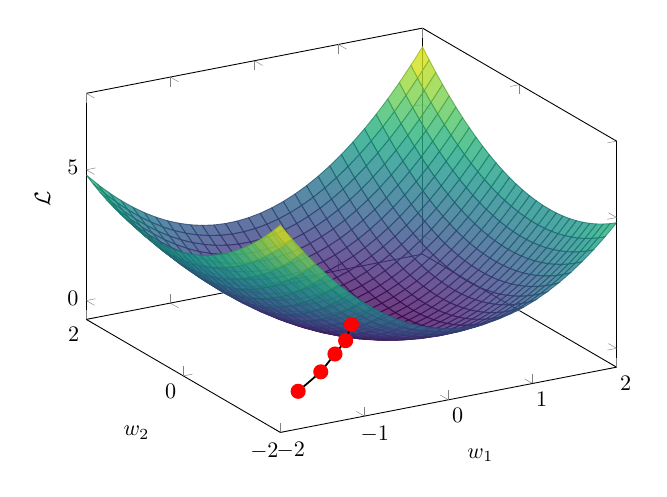
\begin{tikzpicture}[scale=0.8]
        \begin{axis}[
            view={-30}{30},
            xlabel=$w_1$,
            ylabel=$w_2$,
            zlabel=$\mathcal{L}$,
            width=10cm,
            height=8cm
        ]
            % 损失表面近似
            \addplot3[
                surf,
                colormap/viridis,
                samples=30,
                domain=-2:2,
                opacity=0.8
            ] {x^2 + 0.5*y^2 + 0.3*x*y};
            
            % 梯度下降路径
            \addplot3[
                thick,
                black,
                mark=*,
                mark options={red, scale=1.5}
            ] coordinates {
                (-1.5, -1.5, 0)
                (-1.0, -1.1, 0)
                (-0.6, -0.7, 0)
                (-0.3, -0.4, 0)
                (0, 0, 0)
            };
        \end{axis}
    \end{tikzpicture}
    \caption{二次损失表面上的梯度下降}
    \label{fig:gd_quadratic}
\end{figure}

\subsection{优化中的挑战}

\begin{itemize}
    \item \textbf{局部最小值：} 损失景观是非凸的，包含许多局部最小值。然而，对于大型神经网络，局部最小值通常不是大问题；鞍点更常见。
    
    \item \textbf{梯度消失/爆炸：} 在深度网络中，梯度可能变得非常小（消失）或非常大（爆炸），使训练困难。
    
    \item \textbf{平台期：} 梯度接近零的平坦区域，导致进展缓慢。
    
    \item \textbf{损失景观：} 神经网络损失景观复杂，包含许多局部最小值、鞍点和平坦区域。
\end{itemize}

\begin{figure}[htbp]
    \centering
    \begin{tikzpicture}[scale=0.8]
        % 绘制损失景观示意图
        \draw[->] (-3, 0) -- (3, 0) node[right] {参数};
        \draw[->] (0, -0.5) -- (0, 3) node[above] {损失};
        
        % 损失曲线
        \draw[thick, blue] (-2.5, 2.5) to[out=-10, in=170] (-1.5, 1.2) 
            to[out=-20, in=150] (-0.8, 0.3) 
            to[out=-30, in=160] (-0.2, 0.8)  % 局部最小值
            to[out=20, in=180] (0.5, 0.2)
            to[out=0, in=200] (1.5, 0.1)  % 全局最小值
            to[out=20, in=150] (2.5, 0.8);
            
        % 标记全局最小值
        \fill (1.5, 0.1) circle (2pt) node[below] {全局最小};
        
        % 标记局部最小值
        \fill (-0.2, 0.8) circle (2pt) node[above left] {局部最小};
        
        % 标记鞍点
        \fill (-1.2, 0.5) circle (2pt) node[above] {鞍点};
    \end{tikzpicture}
    \caption{包含局部和全局最小值的损失景观示意图}
    \label{fig:loss_landscape}
\end{figure}

\section{信息论}

信息论为理解损失函数（特别是交叉熵）提供了框架。

\subsection{熵}

\begin{定义}[香农熵]
对于具有概率分布 $p(x)$ 的离散随机变量 $X$：
\begin{equation}
H(X) = -\sum_{x} p(x) \log p(x) = E[-\log p(X)]
\end{equation}
熵衡量分布的``不确定性''或``信息量''。对数底数通常是 2（比特）或 $e$（奈特，自然单位）。
\end{定义}

\textbf{历史背景：} 克劳德·香农在他 1948 年的论文《通信的数学理论》\cite{shannon1948mathematical}中引入了熵，创立了信息论。关键洞察是熵提供了满足自然 desiderata（连续性、对等概率结果的单调性以及独立事件的加性）的不确定性的\textbf{唯一}（常数倍）度量。

\subsubsection{证明：通过 Jensen 不等式证明 \texorpdfstring{$D_{KL}(p \| q) \geq 0$}{D_KL(p || q) >= 0}}

KL 散度的非负性是信息论中最重要的结果之一，直接由 Jensen 不等式得出。

\begin{定理}[Jensen 不等式]
对于凸函数 $\phi$ 和随机变量 $X$：
\begin{equation}
\phi(E[X]) \leq E[\phi(X)]
\end{equation}
对于凹函数，不等式反向。相等当且仅当 $X$ 是确定性的（几乎处处常数）或 $\phi$ 在 $X$ 的支撑上是仿射的。
\end{定理}

\begin{证明}[KL 散度的非负性]
由于 $-\log$ 是严格凸函数，根据 Jensen 不等式：
\begin{align}
-D_{KL}(p \| q) &= \sum_x p(x) \log \frac{q(x)}{p(x)} \\
&= E_{p}\left[\log \frac{q}{p}\right] \\
&\leq \log E_{p}\left[\frac{q}{p}\right] \quad \text{（Jensen 不等式，$\log$ 是凹的）} \\
&= \log \left(\sum_x p(x) \frac{q(x)}{p(x)}\right) \\
&= \log \left(\sum_x q(x)\right) = \log 1 = 0
\end{align}
因此 $D_{KL}(p \| q) \geq 0$，当且仅当 $p = q$ 几乎处处相等时等号成立。
\end{证明}

这个证明优雅但有力：它告诉我们交叉熵 $H(p, q)$ 始终至少与真实熵 $H(p)$ 一样大，差距正好是 $D_{KL}(p \| q)$。

\begin{figure}[htbp]
    \centering
    \begin{tikzpicture}[scale=0.9]
        \begin{axis}[
            xlabel={$x$},
            ylabel={$\phi(x)$},
            width=10cm,
            height=6cm,
            domain=0.1:4,
            samples=100,
            legend pos=north east,
            ymin=0, ymax=3,
        ]
            % 凸函数（负对数）
            \addplot[thick, blue] {-ln(x)};
            \addlegendentry{$\phi(x) = -\log x$（凸）}
            % 弦线
            \addplot[thick, red, dashed] coordinates {(0.5, 0.693) (3, -1.099)};
            \node[red] at (axis cs:2.3, 0.4) {弦（割线）};
            % 点
            \addplot[only marks, mark=*, mark size=3pt, black] coordinates {(0.5, 0.693) (3, -1.099)};
            % E[X] 在曲线上的点
            \addplot[only marks, mark=square*, mark size=3pt, green!60!black] coordinates {(1.75, -0.560)};
            \node[green!60!black] at (axis cs:1.75, -0.9) {$\phi(E[X])$};
            % E[phi(X)] 在弦上的点
            \addplot[only marks, mark=triangle*, mark size=3pt, orange] coordinates {(1.75, -0.203)};
            \node[orange] at (axis cs:1.75, 0.05) {$E[\phi(X)]$};
            % 箭头
            \draw[<->, thick, gray] (axis cs:1.95, -0.560) -- (axis cs:1.95, -0.203);
        \end{axis}
    \end{tikzpicture}
    \caption[Jensen 不等式可视化]{凸函数 $\phi(x) = -\log x$ 的 Jensen 不等式：在均值 $E[X]$ 处求值的函数位于期望值 $E[\phi(X)]$ 之下。}
    \label{fig:jensen}
\end{figure}

\subsubsection{互信息}

\begin{定义}[互信息]
两个随机变量 $X$ 和 $Y$ 之间的互信息为：
\begin{equation}
I(X; Y) = D_{KL}(p(x, y) \| p(x)p(y)) = \sum_{x,y} p(x, y) \log \frac{p(x, y)}{p(x)p(y)}
\end{equation}
\end{定义}

互信息满足：
\begin{align}
I(X; Y) &= H(X) - H(X \mid Y) = H(Y) - H(Y \mid X) \\
I(X; Y) &= H(X) + H(Y) - H(X, Y) \\
I(X; Y) &\geq 0 \quad \text{当且仅当 } X \perp Y \text{ 时等号成立}
\end{align}

\textbf{深度学习中的应用：}
\begin{itemize}
    \item \textbf{InfoNCE 损失}（第 3 章）：对比学习最大化同一图像增强视图之间的互信息。
    \item \textbf{信息瓶颈理论} \cite{tishby2015deep}：深度学习被视为将输入 $\mathbf{X}$ 逐步压缩为保留关于目标 $\mathbf{Y}$ 最大信息的表示 $\mathbf{T}$：
    \begin{equation}
    \min_{p(\mathbf{t}|\mathbf{x})} \; I(\mathbf{X}; \mathbf{T}) - \beta I(\mathbf{T}; \mathbf{Y})
    \end{equation}
    \item \textbf{VAE} \cite{kingma2013auto}：证据下界（ELBO）可以写为：
    \begin{equation}
    \log p(\mathbf{x}) \geq \mathbb{E}_{q(\mathbf{z}|\mathbf{x})}[\log p(\mathbf{x}|\mathbf{z})] - D_{KL}(q(\mathbf{z}|\mathbf{x}) \| p(\mathbf{z}))
    \end{equation}
\end{itemize}

\begin{性质}[熵的性质]
\begin{itemize}
    \item 对所有分布 $H(X) \geq 0$
    \item 当且仅当对某个 $x$ 有 $p(x) = 1$ 时 $H(X) = 0$（确定性）
    \item $H(X)$ 在均匀分布时最大化
    \item 二元熵：$H_b(p) = -p\log p - (1-p)\log(1-p)$
\end{itemize}
\end{性质}

\subsection{交叉熵与 KL 散度}

\begin{定义}[交叉熵]
对于两个概率分布 $p$（真实）和 $q$（预测）：
\begin{equation}
H(p, q) = -\sum_{x} p(x) \log q(x) = H(p) + D_{KL}(p \| q)
\end{equation}
\end{定义}

\begin{定义}[KL 散度]
\begin{equation}
D_{KL}(p \| q) = \sum_{x} p(x) \log \frac{p(x)}{q(x)}
\end{equation}
KL 散度衡量从 $q$ 到 $p$ 的``距离''（不是真正的度量，因为它是非对称的）。
\end{定义}

\begin{性质}[KL 散度性质]
\begin{itemize}
    \item $D_{KL}(p \| q) \geq 0$（非负性）
    \item 当且仅当 $p = q$ 时 $D_{KL}(p \| q) = 0$
    \item $D_{KL}(p \| q) \neq D_{KL}(q \| p)$（非对称）
\end{itemize}
\end{性质}

\begin{示例}[交叉熵损失]
对于 $N$ 个样本和 $K$ 个类的分类：
\begin{equation}
\mathcal{L}_{CE} = -\frac{1}{N}\sum_{i=1}^{N}\sum_{k=1}^{K} y_{ik} \log \hat{y}_{ik}
\end{equation}
其中 $y_{ik}$ 是真实标签（独热），$\hat{y}_{ik} = \text{softmax}(z_{ik})$ 是预测。

最小化交叉熵等价于最小化真实分布与预测分布之间的 KL 散度，因为对于独热标签 $H(p)$ 是常数。

\textbf{推导 softmax--交叉熵梯度：} 这是深度学习中最重要的推导之一。对于真实类为 $c$ 的单个样本（独热：$y_c = 1$，$y_{k \neq c} = 0$）：
\begin{align}
\mathcal{L} &= -\sum_{k=1}^{K} y_k \log \hat{y}_k = -\log \hat{y}_c = -\log \frac{e^{z_c}}{\sum_j e^{z_j}} = -z_c + \log \sum_j e^{z_j} \\
\frac{\partial \mathcal{L}}{\partial z_k} &= -y_k + \frac{e^{z_k}}{\sum_j e^{z_j}} = \hat{y}_k - y_k
\end{align}
这个非常简洁的梯度——预测减目标——是分类训练的基石。Softmax 与交叉熵对数``抵消''，避免了分别计算它们时出现的数值问题。
\end{示例}

\section{本章小结}

本章涵盖了神经网络的基本数学基础：

\begin{enumerate}
    \item \textbf{线性代数：} 向量、矩阵、张量运算和范数是在神经网络中表示和操作数据和参数的构建块。
    
    \item \textbf{微积分：} 导数、梯度和链式规则是计算反向传播梯度的基本工具。
    
    \item \textbf{概率论：} 分布、期望值和贝叶斯规则为理解预测和设计损失函数提供了框架。
    
    \item \textbf{优化：} 梯度下降及其变体是神经网络训练的主力。
    
    \item \textbf{信息论：} 熵和 KL 散度为使用交叉熵损失提供了正当理由。
\end{enumerate}

这些数学工具将在整本教材中应用，因为我们探索激活函数、损失函数、网络架构和训练算法。

\section{扩展阅读}

更深入地覆盖这些主题：

\begin{itemize}
    \item \cite{bishop2006pattern} - 线性代数和概率的全面处理
    \item \cite{strang2009introduction} - 线性代数的优秀介绍
    \item \cite{cover2012elements} - 信息论的经典文本
    \item \cite{kingma2013auto} - 变分推断与 ELBO
    \item \cite{tishby2015deep} - 深度学习的信息瓶颈理论
    \item \cite{choriomanska2015loss} - 神经网络损失表面分析
    \item \cite{goodfellow2016deep} - 第 2 章涵盖深度学习的数学基础
    \item \cite{hu2021lora} - 现代模型中的低秩适应和低秩结构
\end{itemize}

% ==============================================================================
% 练习
% ==============================================================================

\section{练习}

\begin{enumerate}
    \item \textbf{线性代数：} 给定权重矩阵 $\mathbf{W} \in \mathbb{R}^{256 \times 512}$，如果我们包含偏置项，这一层有多少参数？写出单次前向传递的计算成本（FLOPs）。
    
    \item \textbf{微积分：} 计算单层网络的梯度 $\frac{\partial \mathcal{L}}{\partial \mathbf{W}}$，输出为 $\mathbf{y} = \mathbf{W}\mathbf{x}$，其中 $\mathcal{L} = \|\mathbf{y} - \mathbf{t}\|^2$。
    
    \item \textbf{概率：} 证明 softmax 函数对加性常数不变：$\text{softmax}(\mathbf{z} + c) = \text{softmax}(\mathbf{z})$ 对任意常数 $c$。
    
    \item \textbf{优化：} 为简单二次函数 $f(x) = x^2$ 实现梯度下降，并分析不同学习率的影响。
    
    \item \textbf{信息论：} 使用 Jensen 不等式证明 $D_{KL}(p \| q) \geq 0$。
\end{enumerate}
